\documentclass[12pt,ngerman]{scrartcl}

\usepackage[utf8]{inputenc}
\usepackage[T1]{fontenc}
\usepackage{babel}
\usepackage{tikz}

\usepackage{siunitx}

\begin{document}
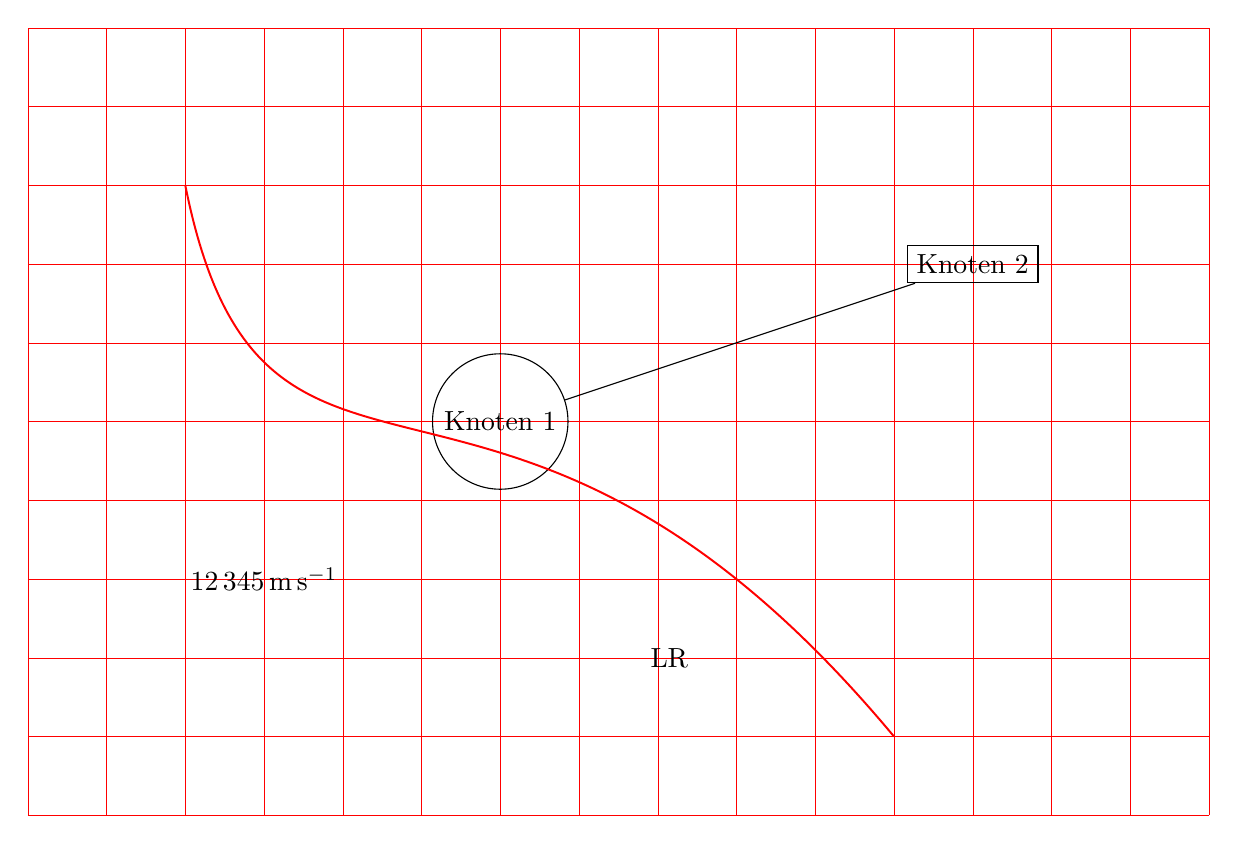
\begin{tikzpicture}
\draw[help lines,red,ultra thin] (0,0) grid (15,10);

\node[draw,circle](K) at (6,5){Knoten 1};
\node[draw](L) at (12,7){Knoten 2};

\draw(K) -- (L);

\node(M)[right] at (8,2){R};
\node[left] at (M){L};

\node(S) at (3,3){\SI{12345}{\meter\per\second}};

\draw[line width =0.25mm,red](2,8) .. controls (3,3) and (6,7) .. (11,1);

\end{tikzpicture}

\end{document}

